% Options for packages loaded elsewhere
% Options for packages loaded elsewhere
\PassOptionsToPackage{unicode}{hyperref}
\PassOptionsToPackage{hyphens}{url}
\PassOptionsToPackage{dvipsnames,svgnames,x11names}{xcolor}
%
\documentclass[
  spanish,
  a4paper,
  oneside]{scrbook}
\usepackage{xcolor}
\usepackage[top=25mm,bottom=25mm,left=30mm,right=20mm]{geometry}
\usepackage{amsmath,amssymb}
\setcounter{secnumdepth}{5}
\usepackage{iftex}
\ifPDFTeX
  \usepackage[T1]{fontenc}
  \usepackage[utf8]{inputenc}
  \usepackage{textcomp} % provide euro and other symbols
\else % if luatex or xetex
  \usepackage{unicode-math} % this also loads fontspec
  \defaultfontfeatures{Scale=MatchLowercase}
  \defaultfontfeatures[\rmfamily]{Ligatures=TeX,Scale=1}
\fi
\usepackage{lmodern}
\ifPDFTeX\else
  % xetex/luatex font selection
\fi
% Use upquote if available, for straight quotes in verbatim environments
\IfFileExists{upquote.sty}{\usepackage{upquote}}{}
\IfFileExists{microtype.sty}{% use microtype if available
  \usepackage[]{microtype}
  \UseMicrotypeSet[protrusion]{basicmath} % disable protrusion for tt fonts
}{}
\makeatletter
\@ifundefined{KOMAClassName}{% if non-KOMA class
  \IfFileExists{parskip.sty}{%
    \usepackage{parskip}
  }{% else
    \setlength{\parindent}{0pt}
    \setlength{\parskip}{6pt plus 2pt minus 1pt}}
}{% if KOMA class
  \KOMAoptions{parskip=half}}
\makeatother
% Make \paragraph and \subparagraph free-standing
\makeatletter
\ifx\paragraph\undefined\else
  \let\oldparagraph\paragraph
  \renewcommand{\paragraph}{
    \@ifstar
      \xxxParagraphStar
      \xxxParagraphNoStar
  }
  \newcommand{\xxxParagraphStar}[1]{\oldparagraph*{#1}\mbox{}}
  \newcommand{\xxxParagraphNoStar}[1]{\oldparagraph{#1}\mbox{}}
\fi
\ifx\subparagraph\undefined\else
  \let\oldsubparagraph\subparagraph
  \renewcommand{\subparagraph}{
    \@ifstar
      \xxxSubParagraphStar
      \xxxSubParagraphNoStar
  }
  \newcommand{\xxxSubParagraphStar}[1]{\oldsubparagraph*{#1}\mbox{}}
  \newcommand{\xxxSubParagraphNoStar}[1]{\oldsubparagraph{#1}\mbox{}}
\fi
\makeatother

\usepackage{color}
\usepackage{fancyvrb}
\newcommand{\VerbBar}{|}
\newcommand{\VERB}{\Verb[commandchars=\\\{\}]}
\DefineVerbatimEnvironment{Highlighting}{Verbatim}{commandchars=\\\{\}}
% Add ',fontsize=\small' for more characters per line
\usepackage{framed}
\definecolor{shadecolor}{RGB}{241,243,245}
\newenvironment{Shaded}{\begin{snugshade}}{\end{snugshade}}
\newcommand{\AlertTok}[1]{\textcolor[rgb]{0.68,0.00,0.00}{#1}}
\newcommand{\AnnotationTok}[1]{\textcolor[rgb]{0.37,0.37,0.37}{#1}}
\newcommand{\AttributeTok}[1]{\textcolor[rgb]{0.40,0.45,0.13}{#1}}
\newcommand{\BaseNTok}[1]{\textcolor[rgb]{0.68,0.00,0.00}{#1}}
\newcommand{\BuiltInTok}[1]{\textcolor[rgb]{0.00,0.23,0.31}{#1}}
\newcommand{\CharTok}[1]{\textcolor[rgb]{0.13,0.47,0.30}{#1}}
\newcommand{\CommentTok}[1]{\textcolor[rgb]{0.37,0.37,0.37}{#1}}
\newcommand{\CommentVarTok}[1]{\textcolor[rgb]{0.37,0.37,0.37}{\textit{#1}}}
\newcommand{\ConstantTok}[1]{\textcolor[rgb]{0.56,0.35,0.01}{#1}}
\newcommand{\ControlFlowTok}[1]{\textcolor[rgb]{0.00,0.23,0.31}{\textbf{#1}}}
\newcommand{\DataTypeTok}[1]{\textcolor[rgb]{0.68,0.00,0.00}{#1}}
\newcommand{\DecValTok}[1]{\textcolor[rgb]{0.68,0.00,0.00}{#1}}
\newcommand{\DocumentationTok}[1]{\textcolor[rgb]{0.37,0.37,0.37}{\textit{#1}}}
\newcommand{\ErrorTok}[1]{\textcolor[rgb]{0.68,0.00,0.00}{#1}}
\newcommand{\ExtensionTok}[1]{\textcolor[rgb]{0.00,0.23,0.31}{#1}}
\newcommand{\FloatTok}[1]{\textcolor[rgb]{0.68,0.00,0.00}{#1}}
\newcommand{\FunctionTok}[1]{\textcolor[rgb]{0.28,0.35,0.67}{#1}}
\newcommand{\ImportTok}[1]{\textcolor[rgb]{0.00,0.46,0.62}{#1}}
\newcommand{\InformationTok}[1]{\textcolor[rgb]{0.37,0.37,0.37}{#1}}
\newcommand{\KeywordTok}[1]{\textcolor[rgb]{0.00,0.23,0.31}{\textbf{#1}}}
\newcommand{\NormalTok}[1]{\textcolor[rgb]{0.00,0.23,0.31}{#1}}
\newcommand{\OperatorTok}[1]{\textcolor[rgb]{0.37,0.37,0.37}{#1}}
\newcommand{\OtherTok}[1]{\textcolor[rgb]{0.00,0.23,0.31}{#1}}
\newcommand{\PreprocessorTok}[1]{\textcolor[rgb]{0.68,0.00,0.00}{#1}}
\newcommand{\RegionMarkerTok}[1]{\textcolor[rgb]{0.00,0.23,0.31}{#1}}
\newcommand{\SpecialCharTok}[1]{\textcolor[rgb]{0.37,0.37,0.37}{#1}}
\newcommand{\SpecialStringTok}[1]{\textcolor[rgb]{0.13,0.47,0.30}{#1}}
\newcommand{\StringTok}[1]{\textcolor[rgb]{0.13,0.47,0.30}{#1}}
\newcommand{\VariableTok}[1]{\textcolor[rgb]{0.07,0.07,0.07}{#1}}
\newcommand{\VerbatimStringTok}[1]{\textcolor[rgb]{0.13,0.47,0.30}{#1}}
\newcommand{\WarningTok}[1]{\textcolor[rgb]{0.37,0.37,0.37}{\textit{#1}}}

\usepackage{longtable,booktabs,array}
\newcounter{none} % for unnumbered tables
\usepackage{calc} % for calculating minipage widths
% Correct order of tables after \paragraph or \subparagraph
\usepackage{etoolbox}
\makeatletter
\patchcmd\longtable{\par}{\if@noskipsec\mbox{}\fi\par}{}{}
\makeatother
% Allow footnotes in longtable head/foot
\IfFileExists{footnotehyper.sty}{\usepackage{footnotehyper}}{\usepackage{footnote}}
\makesavenoteenv{longtable}
\usepackage{graphicx}
\makeatletter
\newsavebox\pandoc@box
\newcommand*\pandocbounded[1]{% scales image to fit in text height/width
  \sbox\pandoc@box{#1}%
  \Gscale@div\@tempa{\textheight}{\dimexpr\ht\pandoc@box+\dp\pandoc@box\relax}%
  \Gscale@div\@tempb{\linewidth}{\wd\pandoc@box}%
  \ifdim\@tempb\p@<\@tempa\p@\let\@tempa\@tempb\fi% select the smaller of both
  \ifdim\@tempa\p@<\p@\scalebox{\@tempa}{\usebox\pandoc@box}%
  \else\usebox{\pandoc@box}%
  \fi%
}
% Set default figure placement to htbp
\def\fps@figure{htbp}
\makeatother


% definitions for citeproc citations
\NewDocumentCommand\citeproctext{}{}
\NewDocumentCommand\citeproc{mm}{%
  \begingroup\def\citeproctext{#2}\cite{#1}\endgroup}
\makeatletter
 % allow citations to break across lines
 \let\@cite@ofmt\@firstofone
 % avoid brackets around text for \cite:
 \def\@biblabel#1{}
 \def\@cite#1#2{{#1\if@tempswa , #2\fi}}
\makeatother
\newlength{\cslhangindent}
\setlength{\cslhangindent}{1.5em}
\newlength{\csllabelwidth}
\setlength{\csllabelwidth}{3em}
\newenvironment{CSLReferences}[2] % #1 hanging-indent, #2 entry-spacing
 {\begin{list}{}{%
  \setlength{\itemindent}{0pt}
  \setlength{\leftmargin}{0pt}
  \setlength{\parsep}{0pt}
  % turn on hanging indent if param 1 is 1
  \ifodd #1
   \setlength{\leftmargin}{\cslhangindent}
   \setlength{\itemindent}{-1\cslhangindent}
  \fi
  % set entry spacing
  \setlength{\itemsep}{#2\baselineskip}}}
 {\end{list}}
\usepackage{calc}
\newcommand{\CSLBlock}[1]{\hfill\break\parbox[t]{\linewidth}{\strut\ignorespaces#1\strut}}
\newcommand{\CSLLeftMargin}[1]{\parbox[t]{\csllabelwidth}{\strut#1\strut}}
\newcommand{\CSLRightInline}[1]{\parbox[t]{\linewidth - \csllabelwidth}{\strut#1\strut}}
\newcommand{\CSLIndent}[1]{\hspace{\cslhangindent}#1}

\ifLuaTeX
\usepackage[bidi=basic,shorthands=off]{babel}
\else
\usepackage[bidi=default,shorthands=off]{babel}
\fi
\ifLuaTeX
  \usepackage{selnolig} % disable illegal ligatures
\fi


\setlength{\emergencystretch}{3em} % prevent overfull lines

\providecommand{\tightlist}{%
  \setlength{\itemsep}{0pt}\setlength{\parskip}{0pt}}



 


\AtBeginDocument{\hypersetup{linkcolor=black}}
% ---------- Paquetes tipograficos y microajustes ----------
\usepackage{microtype}        % mejor interletrado y justificado
\usepackage{csquotes}         % comillas tipograficas
\usepackage{iftex}
\ifPDFTeX\else
  % Seleccion de fuentes solo cuando XeTeX/LuaTeX esta disponible.
  \IfFontExistsTF{TeX Gyre Termes}{
    \setmainfont{TeX Gyre Termes}
  }{
    \IfFontExistsTF{Latin Modern Roman}{\setmainfont{Latin Modern Roman}}{}
  }
  \IfFontExistsTF{TeX Gyre Heros}{
    \setsansfont{TeX Gyre Heros}
  }{
    \IfFontExistsTF{Latin Modern Sans}{\setsansfont{Latin Modern Sans}}{}
  }
  \IfFontExistsTF{TeX Gyre Cursor}{
    \setmonofont{TeX Gyre Cursor}
  }{
    \IfFontExistsTF{Latin Modern Mono}{\setmonofont{Latin Modern Mono}}{}
  }
\fi
\usepackage{enumitem}         % listas compactas
\setlist{itemsep=.2em, topsep=.2em}

% ---------- KOMA-Script: estilo de titulos y espaciado ----------
\KOMAoptions{
  headings=big,
  parskip=half,
  fontsize=12pt,
  appendixprefix=true
}
\setlength{\parindent}{1.5em}
\setlength{\parskip}{0.6em}
\usepackage{indentfirst}
\usepackage{setspace}         % Control del interlineado del documento
\setstretch{1.5}

% ---------- Encabezados y pies (scrlayer-scrpage) ----------
\usepackage[automark,headsepline]{scrlayer-scrpage}
\clearpairofpagestyles
\automark[chapter]{chapter}
\ihead{\pagemark}
\ohead{\itshape\headmark}
\setheadsepline{0.4pt}
\renewcommand*{\chaptermarkformat}{}
\renewcommand*{\chapterpagestyle}{scrheadings}
\pagestyle{scrheadings}
\makeatletter
\let\ps@plain\ps@scrheadings
\makeatother
\cfoot{}

% ---------- Hipervinculos mas sobrios ----------
\usepackage{hyperref}
\hypersetup{
  colorlinks=true,
  linkcolor=black,
  citecolor=[rgb]{0.05,0.2,0.5},
  urlcolor=[rgb]{0.05,0.2,0.5},
  pdfauthor={\@author},
  pdftitle={\@title}
}

% ---------- Leyendas de figuras/tablas ----------
\usepackage[labelfont=bf,textfont=it]{caption}
\captionsetup{
  skip=8pt
}

% ---------- Tabla de contenidos ----------
\KOMAoptions{toc=graduated}
\RedeclareSectionCommand[tocnumwidth=3em]{chapter}
\RedeclareSectionCommand[tocindent=3.25em,tocnumwidth=2.8em]{section}
\RedeclareSectionCommand[tocindent=6.5em,tocnumwidth=2.5em]{subsection}
\makeatletter
\newcommand*{\tocdotfill}{\leavevmode\leaders\hbox to .6em{\hss.\hss}\hfill}
\makeatother
\RedeclareSectionCommand[toclinefill=\tocdotfill]{chapter}
\RedeclareSectionCommand[toclinefill=\tocdotfill]{section}
\RedeclareSectionCommand[toclinefill=\tocdotfill]{subsection}
\renewcommand*{\contentsname}{Tabla de contenido}
\setkomafont{chapterentry}{\normalfont}
\setkomafont{chapterentrypagenumber}{\normalfont}

% ---------- Viudas/Huerfanas y cortes de pagina ----------
\clubpenalty=10000
\widowpenalty=10000
\displaywidowpenalty=10000

% ---------- Entorno abstract para scrbook ----------
\providecommand{\abstractname}{Resumen}
\makeatletter
\@ifundefined{abstract}{
  \newenvironment{abstract}{
    \cleardoublepage
    \thispagestyle{plain}
    \null\vfill
    \begin{center}
      {\bfseries\Large \abstractname\par}
    \end{center}\vspace{1em}
    \begingroup
  }{
    \par\endgroup
    \vfill\null
    \cleardoublepage
  }
}{}
\makeatother

% ---------- Soporte de subtitulo desde YAML ----------
\makeatletter
\providecommand{\subtitle}[1]{\gdef\@subtitle{#1}}
\providecommand{\@subtitle}{}
\makeatother

\makeatletter
\newcommand{\facso@iflist}[4]{%
  \begingroup
    \def\addvspace##1{}%
    \def\numberline##1{##1}%
    \def\facso@target{#2}%
    \newcount\facso@entrycount
    \facso@entrycount=0\relax
    \long\def\contentsline##1##2##3{%
      \def\facso@this{##1}%
      \ifx\facso@this\facso@target
        \advance\facso@entrycount\@ne
      \fi
    }%
    \InputIfFileExists{\jobname.#1}{}{}%
  \endgroup
  \ifnum\facso@entrycount>0\relax
    #3%
  \else
    #4%
  \fi}
\renewcommand{\listoffigures}{%
  \facso@iflist{lof}{figure}{%
    \cleardoublepage
    \phantomsection
    \addchap*{Listado de Figuras}%
    \thispagestyle{scrheadings}%
    \markboth{Listado de Figuras}{Listado de Figuras}%
    \addcontentsline{toc}{chapter}{Listado de Figuras}%
    \@starttoc{lof}%
    \cleardoublepage
    \automark[chapter]{chapter}%
  }{}}
\renewcommand{\listoftables}{%
  \facso@iflist{lot}{table}{%
    \cleardoublepage
    \phantomsection
    \addchap*{Listado de Tablas}%
    \thispagestyle{scrheadings}%
    \markboth{Listado de Tablas}{Listado de Tablas}%
    \addcontentsline{toc}{chapter}{Listado de Tablas}%
    \@starttoc{lot}%
    \cleardoublepage
    \automark[chapter]{chapter}%
  }{}}
\makeatother

% --- Desactivar portada y abstract automaticos de Pandoc (PDF) ---
\AtBeginDocument{\let\maketitle\relax}
\renewenvironment{abstract}{}{}
\providecommand{\appendixname}{}
\providecommand{\appendixtocname}{}
\providecommand{\appendixpagename}{}
\renewcommand*{\appendixname}{Anexo}
\renewcommand*{\appendixtocname}{Anexos}
\renewcommand*{\appendixpagename}{Anexos}
\usepackage{booktabs}
\usepackage{longtable}
\usepackage{array}
\usepackage{multirow}
\usepackage{wrapfig}
\usepackage{float}
\usepackage{colortbl}
\usepackage{pdflscape}
\usepackage{tabu}
\usepackage{threeparttable}
\usepackage{threeparttablex}
\usepackage[normalem]{ulem}
\usepackage{makecell}
\usepackage{xcolor}
\makeatletter
\@ifpackageloaded{caption}{}{\usepackage{caption}}
\AtBeginDocument{%
\ifdefined\contentsname
  \renewcommand*\contentsname{Tabla de contenidos}
\else
  \newcommand\contentsname{Tabla de contenidos}
\fi
\ifdefined\listfigurename
  \renewcommand*\listfigurename{Listado de Figuras}
\else
  \newcommand\listfigurename{Listado de Figuras}
\fi
\ifdefined\listtablename
  \renewcommand*\listtablename{Listado de Tablas}
\else
  \newcommand\listtablename{Listado de Tablas}
\fi
\ifdefined\figurename
  \renewcommand*\figurename{Lista de figuras}
\else
  \newcommand\figurename{Lista de figuras}
\fi
\ifdefined\tablename
  \renewcommand*\tablename{Lista de tablas}
\else
  \newcommand\tablename{Lista de tablas}
\fi
}
\@ifpackageloaded{float}{}{\usepackage{float}}
\floatstyle{ruled}
\@ifundefined{c@chapter}{\newfloat{codelisting}{h}{lop}}{\newfloat{codelisting}{h}{lop}[chapter]}
\floatname{codelisting}{Listado}
\newcommand*\listoflistings{\listof{codelisting}{Listado de Listados}}
\makeatother
\makeatletter
\makeatother
\makeatletter
\@ifpackageloaded{caption}{}{\usepackage{caption}}
\@ifpackageloaded{subcaption}{}{\usepackage{subcaption}}
\makeatother
\usepackage{bookmark}
\IfFileExists{xurl.sty}{\usepackage{xurl}}{} % add URL line breaks if available
\urlstyle{same}
% fallback for those not using the hyperref driver hyperxmp:
\makeatletter
\@ifundefined{xmpquote}{\newcommand{\xmpquote}[1]{#1}}{}
\makeatother
\hypersetup{
  pdftitle={Análisis factorial del PVQ-21 de Schwartz en EDUMERCO Adultos},
  pdfauthor={Javiera Álvarez Cárdenas},
  pdflang={es},
  colorlinks=true,
  linkcolor={Maroon},
  filecolor={Maroon},
  citecolor={Blue},
  urlcolor={Blue},
  pdfcreator={LaTeX via pandoc}}


\title{Análisis factorial del PVQ-21 de Schwartz en EDUMERCO Adultos}
\usepackage{etoolbox}
\makeatletter
\providecommand{\subtitle}[1]{% add subtitle to \maketitle
  \apptocmd{\@title}{\par {\large #1 \par}}{}{}
}
\makeatother
\subtitle{Informe de Investigación en Sociología}
\author{Javiera Álvarez Cárdenas}
\date{9 de octubre de 2026}
\begin{document}
\frontmatter
\maketitle

% --- title-pdf.tex personalizado para portada formal ---
\makeatletter
\providecommand{\subtitle}[1]{\gdef\@subtitle{#1}}
\providecommand{\@subtitle}{}
\providecommand{\frontmattercontext}{}
\providecommand{\advisorname}{}
\providecommand{\advisorlabel}{Profesor guia:}
\providecommand{\frontmatterlocation}{}
\InputIfFileExists{includes/cover-config.tex}{}{}

\newcommand{\PrintTitle}{%
  {\sffamily\bfseries\fontsize{24pt}{28pt}\selectfont \@title\par}%
}
\newcommand{\PrintSubtitle}{%
  \begingroup
  \edef\temp{\detokenize{\@subtitle}}%
  \ifx\temp\empty\relax
    % sin subtitulo
  \else
    {\sffamily\bfseries\large \@subtitle\par}%
  \fi
  \endgroup
}
\newcommand{\PrintAuthor}{%
  {\Large\bfseries \@author\par}%
}
\newcommand{\PrintDate}{%
  {\small \@date\par}%
}
\makeatother

\begin{titlepage}
\thispagestyle{empty}
\begin{center}
\vspace*{10mm}

% Logo o imagen institucional

\includegraphics[width=0.35\textwidth]{assets/cover.png}\par
\vspace{12mm}

% Titulo y subtitulo
\PrintTitle
\vspace{6mm}
\PrintSubtitle

\vspace{22mm}
\begingroup
\edef\temp{\detokenize{\frontmattercontext}}%
\ifx\temp\empty\relax
  % sin contexto adicional
\else
  {\normalsize \frontmattercontext\par}
\fi
\endgroup

\vspace{18mm}
\PrintAuthor

\vspace{16mm}
\begingroup
\edef\temp{\detokenize{\advisorname}}%
\ifx\temp\empty\relax
  % sin tutor
\else
  \rule{0.45\textwidth}{0.4pt}\par
  {\small \advisorlabel\ \advisorname\par}
\fi
\endgroup

\vfill
\begingroup
\edef\temp{\detokenize{\frontmatterlocation}}%
\ifx\temp\empty\relax
  % sin ubicacion
\else
  {\small \frontmatterlocation\par}
\fi
\endgroup
\PrintDate

\end{center}
\end{titlepage}

% Preliminares (numeros romanos) y estilo simple
\frontmatter
\pagestyle{scrheadings}

\setcounter{tocdepth}{2} % (o 1/3 segun prefieras)
\tableofcontents
\listoffigures
\listoftables


\mainmatter
\chapter{Presentación y Objetivos}\label{presentaciuxf3n-y-objetivos}

Este informe presenta el análisis factorial de la escala de valores de
Schwartz (PVQ-21) utilizando los datos del estudio EDUMERCO Adultos.

\section{Modelo de valores de
Schwartz}\label{modelo-de-valores-de-schwartz}

Schwartz plantea que las personas comparten diez valores básicos,
organizados en una estructura circular:

\begin{itemize}
\tightlist
\item
  Los valores \textbf{vecinos} son compatibles entre sí.
\item
  Los valores \textbf{opuestos} se encuentran en mayor tensión.
\item
  Los diez valores se agrupan en \textbf{cuatro dimensiones} de orden
  superior: apertura al cambio, autoensalzamiento, conservación y
  autotrascendencia.
\end{itemize}

{\def\LTcaptype{none} % do not increment counter
\begin{longtable}[]{@{}lll@{}}
\toprule\noalign{}
Valor & Ítems del PVQ-21 & Dimensión \\
\midrule\noalign{}
\endhead
\bottomrule\noalign{}
\endlastfoot
Estimulación & 06, 15 & Apertura al cambio \\
Hedonismo & 10, 21 & Apertura al cambio / autoensalzamiento \\
Logro & 04, 13 & Autoensalzamiento \\
Poder & 02, 17 & Autoensalzamiento \\
Seguridad & 05, 14 & Conservación \\
Conformidad & 07, 16 & Conservación \\
Tradición & 09, 20 & Conservación \\
Benevolencia & 12, 18 & Autotrascendencia \\
Universalismo & 03, 08, 19 & Autotrascendencia \\
Autodirección & 01, 11 & Apertura al cambio \\
\end{longtable}
}

El PVQ-21 aplicado en EDUMERCO es una versión corta, con dos ítems por
valor y tres para universalismo (\citeproc{ref-xie2017bookdown}{Xie,
2017}).

\chapter{Preparación de los datos}\label{preparaciuxf3n-de-los-datos}

\section{Carga de los datos}\label{carga-de-los-datos}

Se cargan los datos de EDUMERCO Adultos y se seleccionan los 21 ítems
del PVQ-21 (\texttt{values\_01} a \texttt{values\_21}).

\begin{Shaded}
\begin{Highlighting}[]
\FunctionTok{load}\NormalTok{(}\StringTok{"input/data/completas{-}280125.RData"}\NormalTok{)   }\CommentTok{\# carga el objeto \textasciigrave{}data\textasciigrave{}}

\NormalTok{items }\OtherTok{\textless{}{-}} \FunctionTok{paste0}\NormalTok{(}\StringTok{"values\_"}\NormalTok{, }\FunctionTok{sprintf}\NormalTok{(}\StringTok{"\%02d"}\NormalTok{, }\DecValTok{1}\SpecialCharTok{:}\DecValTok{21}\NormalTok{))}
\end{Highlighting}
\end{Shaded}

\section{Recodificación de datos
perdidos}\label{recodificaciuxf3n-de-datos-perdidos}

Las respuestas 7 (``No sé'') y 8 (``Preferiría no responder'') se
recodifican como \texttt{NA}.

\begin{Shaded}
\begin{Highlighting}[]
\NormalTok{vals }\OtherTok{\textless{}{-}}\NormalTok{ data }\SpecialCharTok{\%\textgreater{}\%}
  \FunctionTok{select}\NormalTok{(}\FunctionTok{all\_of}\NormalTok{(items)) }\SpecialCharTok{\%\textgreater{}\%}
  \FunctionTok{mutate}\NormalTok{(}\FunctionTok{across}\NormalTok{(}\FunctionTok{everything}\NormalTok{(), as.numeric),}
         \FunctionTok{across}\NormalTok{(}\FunctionTok{everything}\NormalTok{(), }\SpecialCharTok{\textasciitilde{}} \FunctionTok{na\_if}\NormalTok{(}\FunctionTok{na\_if}\NormalTok{(.x, }\DecValTok{7}\NormalTok{), }\DecValTok{8}\NormalTok{)))}
\end{Highlighting}
\end{Shaded}

\section{Selección de casos}\label{selecciuxf3n-de-casos}

Se conservan las personas que respondieron al menos 15 de los 21 ítems.

\begin{Shaded}
\begin{Highlighting}[]
\NormalTok{n\_total  }\OtherTok{\textless{}{-}} \FunctionTok{nrow}\NormalTok{(vals)}
\NormalTok{vals     }\OtherTok{\textless{}{-}}\NormalTok{ vals }\SpecialCharTok{\%\textgreater{}\%} \FunctionTok{filter}\NormalTok{(}\FunctionTok{rowSums}\NormalTok{(}\SpecialCharTok{!}\FunctionTok{is.na}\NormalTok{(.)) }\SpecialCharTok{\textgreater{}=} \DecValTok{15}\NormalTok{)}
\NormalTok{n\_usados }\OtherTok{\textless{}{-}} \FunctionTok{nrow}\NormalTok{(vals)}
\end{Highlighting}
\end{Shaded}

Se utilizan 3.357 de 3.484 personas (96,4\%).

\section{Definición de los valores}\label{definiciuxf3n-de-los-valores}

Cada valor de Schwartz se define como el conjunto de ítems que lo miden,
en el orden del círculo teórico.

\begin{Shaded}
\begin{Highlighting}[]
\NormalTok{valores10 }\OtherTok{\textless{}{-}} \FunctionTok{list}\NormalTok{(}
  \AttributeTok{estimulacion  =} \FunctionTok{c}\NormalTok{(}\StringTok{"06"}\NormalTok{, }\StringTok{"15"}\NormalTok{), }\AttributeTok{hedonismo     =} \FunctionTok{c}\NormalTok{(}\StringTok{"10"}\NormalTok{, }\StringTok{"21"}\NormalTok{),}
  \AttributeTok{logro         =} \FunctionTok{c}\NormalTok{(}\StringTok{"04"}\NormalTok{, }\StringTok{"13"}\NormalTok{), }\AttributeTok{poder         =} \FunctionTok{c}\NormalTok{(}\StringTok{"02"}\NormalTok{, }\StringTok{"17"}\NormalTok{),}
  \AttributeTok{seguridad     =} \FunctionTok{c}\NormalTok{(}\StringTok{"05"}\NormalTok{, }\StringTok{"14"}\NormalTok{), }\AttributeTok{conformidad   =} \FunctionTok{c}\NormalTok{(}\StringTok{"07"}\NormalTok{, }\StringTok{"16"}\NormalTok{),}
  \AttributeTok{tradicion     =} \FunctionTok{c}\NormalTok{(}\StringTok{"09"}\NormalTok{, }\StringTok{"20"}\NormalTok{), }\AttributeTok{benevolencia  =} \FunctionTok{c}\NormalTok{(}\StringTok{"12"}\NormalTok{, }\StringTok{"18"}\NormalTok{),}
  \AttributeTok{universalismo =} \FunctionTok{c}\NormalTok{(}\StringTok{"03"}\NormalTok{, }\StringTok{"08"}\NormalTok{, }\StringTok{"19"}\NormalTok{), }\AttributeTok{autodireccion =} \FunctionTok{c}\NormalTok{(}\StringTok{"01"}\NormalTok{, }\StringTok{"11"}\NormalTok{)}
\NormalTok{)}

\NormalTok{nombres }\OtherTok{\textless{}{-}} \FunctionTok{c}\NormalTok{(}\AttributeTok{estimulacion =} \StringTok{"Estimulación"}\NormalTok{, }\AttributeTok{hedonismo =} \StringTok{"Hedonismo"}\NormalTok{,}
             \AttributeTok{logro =} \StringTok{"Logro"}\NormalTok{, }\AttributeTok{poder =} \StringTok{"Poder"}\NormalTok{, }\AttributeTok{seguridad =} \StringTok{"Seguridad"}\NormalTok{,}
             \AttributeTok{conformidad =} \StringTok{"Conformidad"}\NormalTok{, }\AttributeTok{tradicion =} \StringTok{"Tradición"}\NormalTok{,}
             \AttributeTok{benevolencia =} \StringTok{"Benevolencia"}\NormalTok{, }\AttributeTok{universalismo =} \StringTok{"Universalismo"}\NormalTok{,}
             \AttributeTok{autodireccion =} \StringTok{"Autodirección"}\NormalTok{)}
\end{Highlighting}
\end{Shaded}

\section{Versión centrada de las
respuestas}\label{versiuxf3n-centrada-de-las-respuestas}

Se construye además una versión centrada, restando a cada respuesta el
promedio de la persona, para considerar la importancia relativa de los
valores.

\begin{Shaded}
\begin{Highlighting}[]
\NormalTok{vals\_c }\OtherTok{\textless{}{-}}\NormalTok{ vals }\SpecialCharTok{{-}} \FunctionTok{rowMeans}\NormalTok{(vals, }\AttributeTok{na.rm =} \ConstantTok{TRUE}\NormalTok{)}
\end{Highlighting}
\end{Shaded}

\chapter{Estadísticos descriptivos}\label{estaduxedsticos-descriptivos}

\section{Por ítem}\label{por-uxedtem}

\begin{Shaded}
\begin{Highlighting}[]
\NormalTok{descriptivos }\OtherTok{\textless{}{-}}\NormalTok{ psych}\SpecialCharTok{::}\FunctionTok{describe}\NormalTok{(vals)}

\NormalTok{descriptivos }\SpecialCharTok{\%\textgreater{}\%}
  \FunctionTok{select}\NormalTok{(n, mean, sd, min, max, skew, kurtosis) }\SpecialCharTok{\%\textgreater{}\%}
  \FunctionTok{mutate}\NormalTok{(}\FunctionTok{across}\NormalTok{(}\FunctionTok{where}\NormalTok{(is.numeric), }\SpecialCharTok{\textasciitilde{}} \FunctionTok{round}\NormalTok{(.x, }\DecValTok{2}\NormalTok{))) }\SpecialCharTok{\%\textgreater{}\%}
  \FunctionTok{kbl}\NormalTok{(}
    \AttributeTok{col.names =} \FunctionTok{c}\NormalTok{(}\StringTok{"N"}\NormalTok{, }\StringTok{"Media"}\NormalTok{, }\StringTok{"DE"}\NormalTok{, }\StringTok{"Mín."}\NormalTok{, }\StringTok{"Máx."}\NormalTok{, }\StringTok{"Asimetría"}\NormalTok{, }\StringTok{"Curtosis"}\NormalTok{),}
    \AttributeTok{format.args =} \FunctionTok{list}\NormalTok{(}\AttributeTok{big.mark =} \StringTok{"."}\NormalTok{, }\AttributeTok{decimal.mark =} \StringTok{","}\NormalTok{)}
\NormalTok{  ) }\SpecialCharTok{\%\textgreater{}\%}
  \FunctionTok{kable\_styling}\NormalTok{(}\AttributeTok{full\_width =} \ConstantTok{FALSE}\NormalTok{)}
\end{Highlighting}
\end{Shaded}

\begin{table}

\caption{\label{tbl-descriptivos-item}Descriptivos por ítem (escala de 1
a 6)}

\centering{

\centering
\begin{tabular}[t]{l|r|r|r|r|r|r|r}
\hline
  & N & Media & DE & Mín. & Máx. & Asimetría & Curtosis\\
\hline
values\_01 & 3.318 & 3,87 & 1,24 & 1 & 6 & -0,09 & -0,55\\
\hline
values\_02 & 3.335 & 2,44 & 1,26 & 1 & 6 & 0,96 & 0,40\\
\hline
values\_03 & 3.342 & 4,81 & 1,19 & 1 & 6 & -0,93 & 0,19\\
\hline
values\_04 & 3.317 & 2,95 & 1,38 & 1 & 6 & 0,50 & -0,63\\
\hline
values\_05 & 3.334 & 4,78 & 1,23 & 1 & 6 & -0,88 & 0,02\\
\hline
values\_06 & 3.332 & 3,88 & 1,38 & 1 & 6 & -0,09 & -0,90\\
\hline
values\_07 & 3.289 & 3,55 & 1,49 & 1 & 6 & -0,01 & -1,04\\
\hline
values\_08 & 3.339 & 4,32 & 1,21 & 1 & 6 & -0,48 & -0,35\\
\hline
values\_09 & 3.334 & 4,55 & 1,23 & 1 & 6 & -0,61 & -0,35\\
\hline
values\_10 & 3.329 & 3,74 & 1,36 & 1 & 6 & -0,07 & -0,84\\
\hline
values\_11 & 3.336 & 4,55 & 1,26 & 1 & 6 & -0,60 & -0,44\\
\hline
values\_12 & 3.336 & 4,70 & 1,15 & 1 & 6 & -0,66 & -0,28\\
\hline
values\_13 & 3.317 & 3,25 & 1,42 & 1 & 6 & 0,34 & -0,84\\
\hline
values\_14 & 3.308 & 4,77 & 1,33 & 1 & 6 & -0,97 & 0,10\\
\hline
values\_15 & 3.330 & 3,11 & 1,39 & 1 & 6 & 0,38 & -0,70\\
\hline
values\_16 & 3.312 & 4,09 & 1,35 & 1 & 6 & -0,26 & -0,84\\
\hline
values\_17 & 3.298 & 3,35 & 1,41 & 1 & 6 & 0,26 & -0,89\\
\hline
values\_18 & 3.329 & 4,62 & 1,21 & 1 & 6 & -0,69 & -0,14\\
\hline
values\_19 & 3.331 & 4,76 & 1,21 & 1 & 6 & -0,78 & -0,12\\
\hline
values\_20 & 3.310 & 3,68 & 1,53 & 1 & 6 & -0,11 & -1,04\\
\hline
values\_21 & 3.310 & 3,59 & 1,39 & 1 & 6 & 0,07 & -0,87\\
\hline
\end{tabular}

}

\end{table}%

\section{Por valor}\label{por-valor}

\begin{Shaded}
\begin{Highlighting}[]
\NormalTok{tabla\_valores }\OtherTok{\textless{}{-}}\NormalTok{ purrr}\SpecialCharTok{::}\FunctionTok{map\_dfr}\NormalTok{(}
  \FunctionTok{names}\NormalTok{(valores10),}
  \ControlFlowTok{function}\NormalTok{(v) \{}
\NormalTok{    vars }\OtherTok{\textless{}{-}} \FunctionTok{paste0}\NormalTok{(}\StringTok{"values\_"}\NormalTok{, valores10[[v]])}

    \FunctionTok{tibble}\NormalTok{(}
      \AttributeTok{valor =}\NormalTok{ nombres[v],}
      \AttributeTok{puntaje =} \FunctionTok{rowMeans}\NormalTok{(vals[, vars], }\AttributeTok{na.rm =} \ConstantTok{TRUE}\NormalTok{)}
\NormalTok{    )}
\NormalTok{  \}}
\NormalTok{)}

\NormalTok{resumen\_valores }\OtherTok{\textless{}{-}}\NormalTok{ tabla\_valores }\SpecialCharTok{\%\textgreater{}\%}
  \FunctionTok{group\_by}\NormalTok{(valor) }\SpecialCharTok{\%\textgreater{}\%}
  \FunctionTok{summarise}\NormalTok{(}
    \AttributeTok{n        =} \FunctionTok{sum}\NormalTok{(}\SpecialCharTok{!}\FunctionTok{is.na}\NormalTok{(puntaje)),}
    \AttributeTok{promedio =} \FunctionTok{mean}\NormalTok{(puntaje, }\AttributeTok{na.rm =} \ConstantTok{TRUE}\NormalTok{),}
    \AttributeTok{de       =} \FunctionTok{sd}\NormalTok{(puntaje, }\AttributeTok{na.rm =} \ConstantTok{TRUE}\NormalTok{),}
    \AttributeTok{.groups  =} \StringTok{"drop"}
\NormalTok{  ) }\SpecialCharTok{\%\textgreater{}\%}
  \FunctionTok{arrange}\NormalTok{(}\FunctionTok{desc}\NormalTok{(promedio))}

\NormalTok{resumen\_valores }\SpecialCharTok{\%\textgreater{}\%}
  \FunctionTok{mutate}\NormalTok{(}\FunctionTok{across}\NormalTok{(}\FunctionTok{c}\NormalTok{(promedio, de), }\SpecialCharTok{\textasciitilde{}} \FunctionTok{round}\NormalTok{(.x, }\DecValTok{2}\NormalTok{))) }\SpecialCharTok{\%\textgreater{}\%}
  \FunctionTok{kbl}\NormalTok{(}
    \AttributeTok{col.names =} \FunctionTok{c}\NormalTok{(}\StringTok{"Valor"}\NormalTok{, }\StringTok{"N"}\NormalTok{, }\StringTok{"Media"}\NormalTok{, }\StringTok{"DE"}\NormalTok{),}
    \AttributeTok{align =} \StringTok{"lrrr"}\NormalTok{,}
    \AttributeTok{format.args =} \FunctionTok{list}\NormalTok{(}\AttributeTok{big.mark =} \StringTok{"."}\NormalTok{, }\AttributeTok{decimal.mark =} \StringTok{","}\NormalTok{)}
\NormalTok{  ) }\SpecialCharTok{\%\textgreater{}\%}
  \FunctionTok{kable\_styling}\NormalTok{(}\AttributeTok{bootstrap\_options =} \FunctionTok{c}\NormalTok{(}\StringTok{"striped"}\NormalTok{, }\StringTok{"hover"}\NormalTok{), }\AttributeTok{full\_width =} \ConstantTok{FALSE}\NormalTok{)}
\end{Highlighting}
\end{Shaded}

\begin{table}

\caption{\label{tbl-descriptivos-valor}Puntaje promedio por valor
(escala de 1 a 6)}

\centering{

\centering
\begin{tabular}[t]{l|r|r|r}
\hline
Valor & N & Media & DE\\
\hline
Seguridad & 3.354 & 4,77 & 1,08\\
\hline
Benevolencia & 3.352 & 4,66 & 1,00\\
\hline
Universalismo & 3.357 & 4,63 & 0,91\\
\hline
Autodirección & 3.356 & 4,21 & 1,03\\
\hline
Tradición & 3.355 & 4,12 & 1,06\\
\hline
Conformidad & 3.348 & 3,82 & 1,17\\
\hline
Hedonismo & 3.353 & 3,67 & 1,20\\
\hline
Estimulación & 3.353 & 3,50 & 1,19\\
\hline
Logro & 3.349 & 3,10 & 1,25\\
\hline
Poder & 3.355 & 2,90 & 1,08\\
\hline
\end{tabular}

}

\end{table}%

\chapter{Relación entre los
valores}\label{relaciuxf3n-entre-los-valores}

Para esto se usan los puntajes centrados (cada respuesta menos el
promedio de la persona), que es la corrección que recomienda Schwartz.
Al centrar aparecen correlaciones negativas por construcción, así que es
una exploración y no una prueba de la estructura circular.

\begin{Shaded}
\begin{Highlighting}[]
\NormalTok{scores }\OtherTok{\textless{}{-}} \FunctionTok{map\_dfc}\NormalTok{(valores10,}
                  \SpecialCharTok{\textasciitilde{}} \FunctionTok{rowMeans}\NormalTok{(vals\_c[, }\FunctionTok{paste0}\NormalTok{(}\StringTok{"values\_"}\NormalTok{, .x)], }\AttributeTok{na.rm =} \ConstantTok{TRUE}\NormalTok{))}

\NormalTok{R }\OtherTok{\textless{}{-}} \FunctionTok{cor}\NormalTok{(scores, }\AttributeTok{use =} \StringTok{"pairwise.complete.obs"}\NormalTok{)}
\NormalTok{orden }\OtherTok{\textless{}{-}} \FunctionTok{names}\NormalTok{(valores10)}

\FunctionTok{as.data.frame}\NormalTok{(}\FunctionTok{as.table}\NormalTok{(R)) }\SpecialCharTok{\%\textgreater{}\%}
  \FunctionTok{mutate}\NormalTok{(}\AttributeTok{Var1 =} \FunctionTok{factor}\NormalTok{(nombres[}\FunctionTok{as.character}\NormalTok{(Var1)], }\AttributeTok{levels =}\NormalTok{ nombres[orden]),}
         \AttributeTok{Var2 =} \FunctionTok{factor}\NormalTok{(nombres[}\FunctionTok{as.character}\NormalTok{(Var2)], }\AttributeTok{levels =} \FunctionTok{rev}\NormalTok{(nombres[orden]))) }\SpecialCharTok{\%\textgreater{}\%}
  \FunctionTok{ggplot}\NormalTok{(}\FunctionTok{aes}\NormalTok{(Var1, Var2, }\AttributeTok{fill =}\NormalTok{ Freq)) }\SpecialCharTok{+}
  \FunctionTok{geom\_tile}\NormalTok{() }\SpecialCharTok{+}
  \FunctionTok{geom\_text}\NormalTok{(}\FunctionTok{aes}\NormalTok{(}\AttributeTok{label =} \FunctionTok{format}\NormalTok{(}\FunctionTok{round}\NormalTok{(Freq, }\DecValTok{2}\NormalTok{), }\AttributeTok{decimal.mark =} \StringTok{","}\NormalTok{)), }\AttributeTok{size =} \FloatTok{2.8}\NormalTok{) }\SpecialCharTok{+}
  \FunctionTok{scale\_fill\_gradient2}\NormalTok{(}\AttributeTok{low =} \StringTok{"firebrick"}\NormalTok{, }\AttributeTok{mid =} \StringTok{"white"}\NormalTok{, }\AttributeTok{high =} \StringTok{"steelblue"}\NormalTok{,}
                       \AttributeTok{limits =} \FunctionTok{c}\NormalTok{(}\SpecialCharTok{{-}}\DecValTok{1}\NormalTok{, }\DecValTok{1}\NormalTok{)) }\SpecialCharTok{+}
  \FunctionTok{labs}\NormalTok{(}\AttributeTok{x =} \ConstantTok{NULL}\NormalTok{, }\AttributeTok{y =} \ConstantTok{NULL}\NormalTok{, }\AttributeTok{fill =} \StringTok{"r"}\NormalTok{) }\SpecialCharTok{+}
  \FunctionTok{coord\_fixed}\NormalTok{() }\SpecialCharTok{+}
  \FunctionTok{theme\_minimal}\NormalTok{() }\SpecialCharTok{+}
  \FunctionTok{theme}\NormalTok{(}\AttributeTok{axis.text.x =} \FunctionTok{element\_text}\NormalTok{(}\AttributeTok{angle =} \DecValTok{45}\NormalTok{, }\AttributeTok{hjust =} \DecValTok{1}\NormalTok{))}
\end{Highlighting}
\end{Shaded}

\begin{figure}[H]

\caption{\label{fig-correlaciones}Correlaciones entre valores (puntajes
centrados)}

\centering{

\pandocbounded{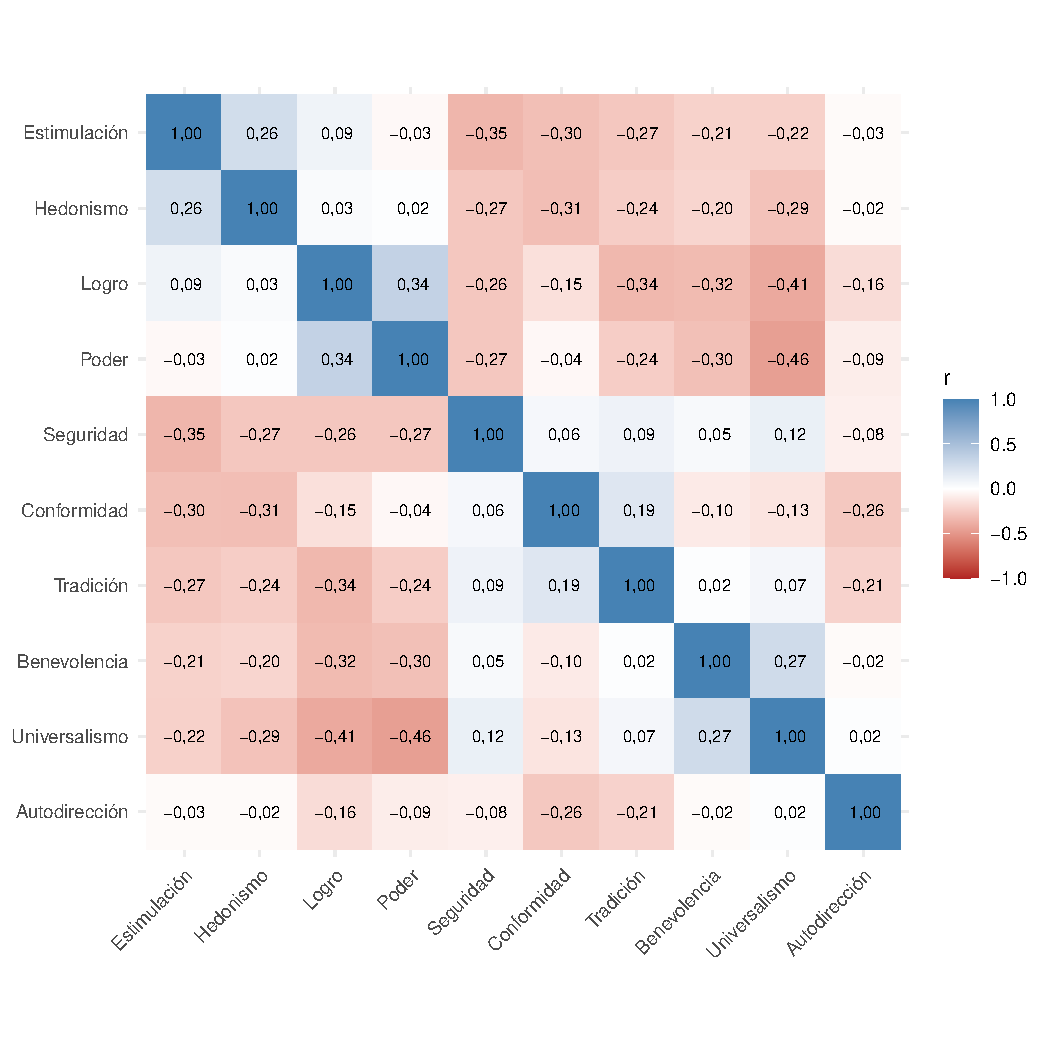
\includegraphics[keepaspectratio]{index_files/figure-pdf/fig-correlaciones-1.pdf}}

}

\end{figure}%

Varios valores vecinos correlacionan positivamente (poder--logro, 0,34;
benevolencia--universalismo, 0,27; estimulación--hedonismo, 0,26;
conformidad--tradición, 0,19) y algunos opuestos correlacionan
negativamente (poder--universalismo, −0,46; logro--universalismo, −0,41;
estimulación--seguridad, −0,35). Autodirección tiene correlaciones
cercanas a cero con casi todos los valores, y seguridad se asocia poco
con conformidad y tradición.

\chapter{Análisis factorial
exploratorio}\label{anuxe1lisis-factorial-exploratorio}

\section{Adecuación de los datos (KMO y
Bartlett)}\label{adecuaciuxf3n-de-los-datos-kmo-y-bartlett}

\begin{Shaded}
\begin{Highlighting}[]
\NormalTok{cor\_poly }\OtherTok{\textless{}{-}}\NormalTok{ psych}\SpecialCharTok{::}\FunctionTok{polychoric}\NormalTok{(vals)}

\NormalTok{kmo   }\OtherTok{\textless{}{-}} \FunctionTok{KMO}\NormalTok{(cor\_poly}\SpecialCharTok{$}\NormalTok{rho)}
\NormalTok{bart  }\OtherTok{\textless{}{-}} \FunctionTok{cortest.bartlett}\NormalTok{(cor\_poly}\SpecialCharTok{$}\NormalTok{rho, }\AttributeTok{n =} \FunctionTok{nrow}\NormalTok{(vals))}
\end{Highlighting}
\end{Shaded}

El índice KMO global fue de 0,88, y la prueba de Bartlett fue
significativa (χ²(210) = 22.614,3, p \textless{} 0,001), por lo que los
datos son adecuados para un análisis factorial.

\section{Número de factores}\label{nuxfamero-de-factores}

\begin{Shaded}
\begin{Highlighting}[]
\NormalTok{pa }\OtherTok{\textless{}{-}} \FunctionTok{fa.parallel}\NormalTok{(cor\_poly}\SpecialCharTok{$}\NormalTok{rho, }\AttributeTok{n.obs =} \FunctionTok{nrow}\NormalTok{(vals), }\AttributeTok{fa =} \StringTok{"fa"}\NormalTok{, }\AttributeTok{fm =} \StringTok{"minres"}\NormalTok{,}
                  \AttributeTok{plot =} \ConstantTok{FALSE}\NormalTok{)}
\end{Highlighting}
\end{Shaded}

\begin{Shaded}
\begin{Highlighting}[]
\FunctionTok{tibble}\NormalTok{(}\AttributeTok{factor =} \FunctionTok{seq\_along}\NormalTok{(pa}\SpecialCharTok{$}\NormalTok{fa.values),}
       \StringTok{\textasciigrave{}}\AttributeTok{Datos observados}\StringTok{\textasciigrave{}} \OtherTok{=}\NormalTok{ pa}\SpecialCharTok{$}\NormalTok{fa.values,}
       \StringTok{\textasciigrave{}}\AttributeTok{Datos simulados (azar)}\StringTok{\textasciigrave{}} \OtherTok{=}\NormalTok{ pa}\SpecialCharTok{$}\NormalTok{fa.sim) }\SpecialCharTok{\%\textgreater{}\%}
  \FunctionTok{pivot\_longer}\NormalTok{(}\SpecialCharTok{{-}}\NormalTok{factor, }\AttributeTok{names\_to =} \StringTok{"serie"}\NormalTok{, }\AttributeTok{values\_to =} \StringTok{"autovalor"}\NormalTok{) }\SpecialCharTok{\%\textgreater{}\%}
  \FunctionTok{ggplot}\NormalTok{(}\FunctionTok{aes}\NormalTok{(factor, autovalor, }\AttributeTok{color =}\NormalTok{ serie, }\AttributeTok{linetype =}\NormalTok{ serie)) }\SpecialCharTok{+}
  \FunctionTok{geom\_line}\NormalTok{() }\SpecialCharTok{+}
  \FunctionTok{geom\_point}\NormalTok{() }\SpecialCharTok{+}
  \FunctionTok{geom\_hline}\NormalTok{(}\AttributeTok{yintercept =} \DecValTok{0}\NormalTok{, }\AttributeTok{color =} \StringTok{"grey70"}\NormalTok{) }\SpecialCharTok{+}
  \FunctionTok{scale\_color\_manual}\NormalTok{(}\AttributeTok{values =} \FunctionTok{c}\NormalTok{(}\StringTok{"Datos observados"} \OtherTok{=} \StringTok{"steelblue"}\NormalTok{,}
                                \StringTok{"Datos simulados (azar)"} \OtherTok{=} \StringTok{"firebrick"}\NormalTok{)) }\SpecialCharTok{+}
  \FunctionTok{scale\_linetype\_manual}\NormalTok{(}\AttributeTok{values =} \FunctionTok{c}\NormalTok{(}\StringTok{"Datos observados"} \OtherTok{=} \StringTok{"solid"}\NormalTok{,}
                                   \StringTok{"Datos simulados (azar)"} \OtherTok{=} \StringTok{"dashed"}\NormalTok{)) }\SpecialCharTok{+}
  \FunctionTok{labs}\NormalTok{(}\AttributeTok{x =} \StringTok{"Número de factor"}\NormalTok{, }\AttributeTok{y =} \StringTok{"Autovalor"}\NormalTok{, }\AttributeTok{color =} \ConstantTok{NULL}\NormalTok{, }\AttributeTok{linetype =} \ConstantTok{NULL}\NormalTok{) }\SpecialCharTok{+}
  \FunctionTok{theme\_minimal}\NormalTok{() }\SpecialCharTok{+}
  \FunctionTok{theme}\NormalTok{(}\AttributeTok{legend.position =} \StringTok{"bottom"}\NormalTok{)}
\end{Highlighting}
\end{Shaded}

\begin{figure}[H]

\caption{\label{fig-analisis-paralelo}Análisis paralelo}

\centering{

\pandocbounded{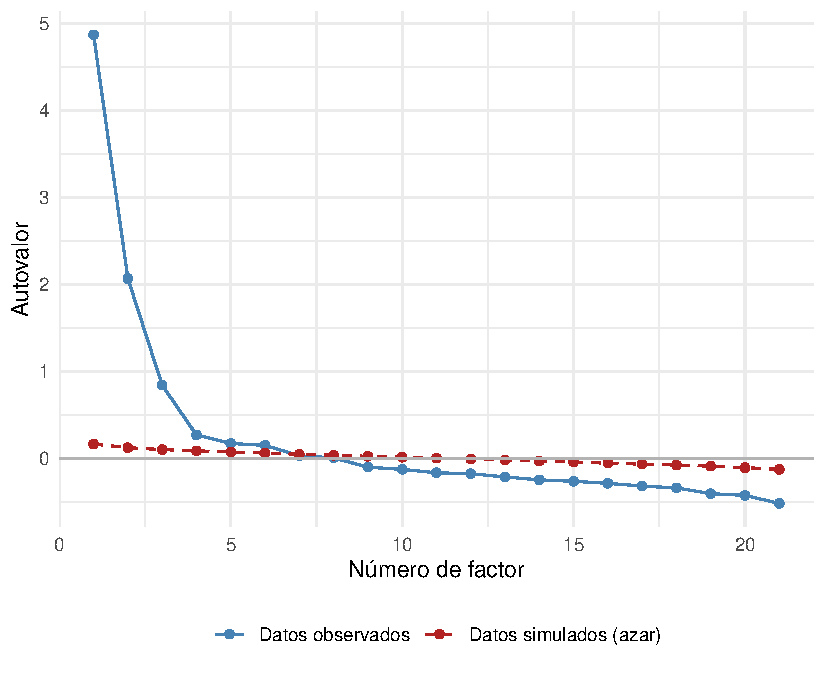
\includegraphics[keepaspectratio]{index_files/figure-pdf/fig-analisis-paralelo-1.pdf}}

}

\end{figure}%

La línea azul son los datos y la roja punteada lo esperable por azar, se
consideran los factores donde la azul queda por encima.

El análisis paralelo sugiere 6 factores.

\chapter*{Referencias}\label{referencias}
\addcontentsline{toc}{chapter}{Referencias}

\protect\phantomsection\label{refs}
\begin{CSLReferences}{1}{0}
\bibitem[\citeproctext]{ref-xie2017bookdown}
Xie, Y. (2017). \emph{bookdown: Authoring Books and Technical Documents
with R Markdown}. Chapman; Hall/CRC.

\end{CSLReferences}


\backmatter

% --- Cuerpo del libro (capítulos) en arábigos ---
\mainmatter
\pagestyle{scrheadings}

% --- (Opcional) Estilo del índice general ---
% \addtocontents{toc}{\protect\thispagestyle{plain}}


\end{document}
